\documentclass[letterpaper,headings=standardclasses,parskip=half]{scrartcl}

% \usepackage[french]{babel}
\usepackage[hmargin=1.25in,vmargin=1in]{geometry}
\usepackage{graphicx}
\usepackage[hidelinks]{hyperref}
\usepackage{listings}
\usepackage{xcolor}

% \usepackage[backend=bibtex]{biblatex}

% \addbibresource{references.bib}

\newcommand{\todo}{{\color{red}{TODO}}}

\titlehead{
    \centering
    
\includegraphics[width=2in]{Signature_electronique 150.jpg}
}
\subject{LOG8415E - Advanced Concepts of Cloud Computing}
\title{Lab 2 – Deploying Webapps on Containers on AWS}
\subtitle{Report}
\author{
    Quentin Guidée (2206809) 
    \and
    Aurel Lucrich Ikama Honey (2160742)
    \and
    Nam Vu (2230468)
}
\date{\today}
\publishers{Polytechnique Montréal – Fall 2023}

\lstdefinestyle{lststyle}{
    basicstyle=\ttfamily
}
\lstset{style=lststyle}

\begin{document}
\maketitle
\thispagestyle{empty}

\clearpage
\pagenumbering{arabic}
\tableofcontents

\clearpage
\section*{Handover Documentation Report}

\subsection*{Project Title}

Cluster Benchmarking using EC2 Virtual Machines and Elastic Load Balancer (ELB)

\subsection*{Report Date}

\today

\subsection*{Team Members}

\begin{itemize}
    \item Quentin Guidée (2206809)
    \item Aurel Lucrich Ikama Honey (2160742)
    \item Nam Vu (2230468)
\end{itemize}

\noindent\rule{\textwidth}{0.3pt}

\section*{Executive Summary}

\todo

\noindent\rule{\textwidth}{0.3pt}

\section{Introduction}

The goal of this second project is to continue experimenting with AWS.
This time, the load balancer will be abstracted by writing a custom orchestrator.
This orchestrator will be responsible for dispatching requests to multiple workers.
Finally, the workers will be used to run inference on machine learning models.

\section{Project objectives}

Different objectives are fixed for this project:
\begin{itemize}
    \item Create and deploy a custom orchestrator on Amazon EC2.
    \item Deploy multiple workers, running by pairs on Amazon EC2.
\end{itemize}

\section{Approach}

First of all, the code from the previous project has been reused, except for the load balancer and the flask app.
This allowed us to quickly have a working solution.

Then, the load balancer has been replaced by a custom orchestrator. This consists of a simple flask app, which dispatches requests to the workers and manages instances state.

Finally, the workers have been deployed. Each EC2 instance runs two workers, which are both listening on different ports.

Like the previous project, all the code is versioned in a Git monorepo. The Python project is managed using the Poetry dependency manager: this makes it easier to manage dependencies across the different subprojects and automate the venv setup.

\section{Tasks and Responsoibilities}

\subsection*{Nam Vu}

\begin{itemize}
    \item Adapt the code from the previous project to the new requirements.
\end{itemize}

\subsection*{Quentin Guidée}

\begin{itemize}
    \item Create the orchestrator.
\end{itemize}

\subsection*{Aurel Lucrich Ikama Honey}

\begin{itemize}
    \item Create the workers.
\end{itemize}

\section{Progress and achievements}

Initially, we took over some of the code from the previous project. We reused the deployment code for the EC2 instances and the Flask application.

As in the previous project, we've created a bootstrap script to build our infrastructure. This script is used to create the EC2 instances in which we've deployed two Docker containers. In each of these containers, we have deployed a flask application.

This Flask application as indicated in the subject calls a function that is responsible for performing inference on an ML model.

In this project we used the machine learning Transformer model called
DistilBERT. This is a reduced but faster version of the BERT model that enables
bidirectional text prediction from a given unlabeled text. EC2 instances are
deployed in a security group that allows SSH and HTTP connections from the
outside. The instances are called workers and there are 4 of them. In short, we
have 4 workers, each containing two docker containers (with a machine learning application). See Figure \ref{fig:infra}.

We then created an orchestrator to dispatch requests to all workers. This orchestrator is a flask application that manages the state of EC2 instances and dispatches requests to all workers.

Finally, to test our infrastructure, we used a test script in the bench module, which executes a given number (here 5) of requests in parallel on the orchestrator. We used the python library \emph{multiprocessing} to create a pool of processes to execute the requests in parallel.

\begin{figure}
    \centering
    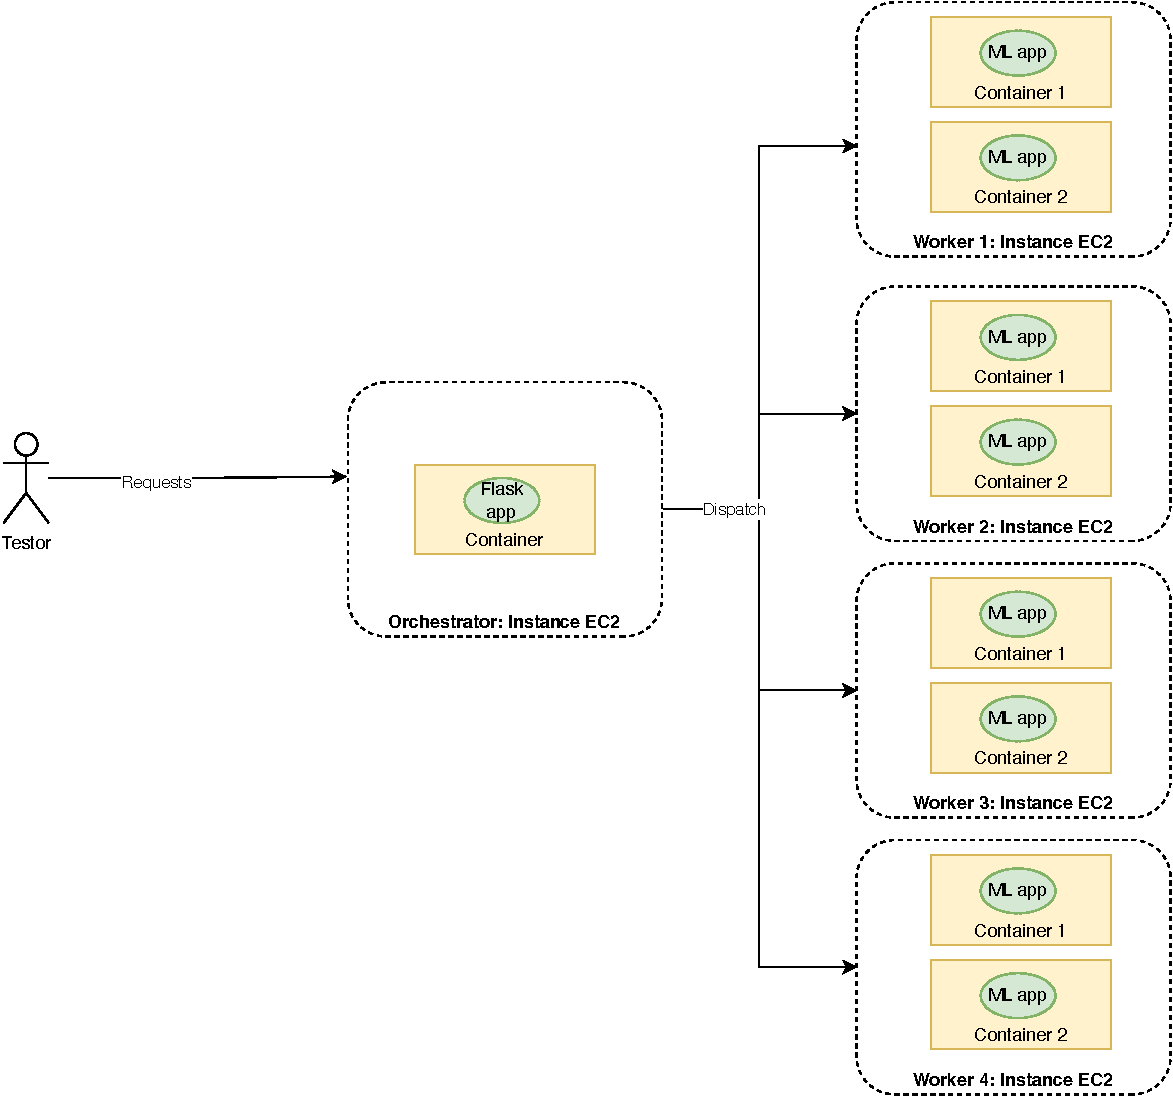
\includegraphics[width=\textwidth]{images/infra.pdf}
    \caption{Infrastructure diagram}
    \label{fig:infra}
\end{figure}


\section{Results and Outcomes}

\todo

\section{Lessons learned}

\begin{itemize}
    \item The code from project 1 was very modular, which made it easy to adapt it to the new requirements. So good code design is important to support future changes.
    \item While the orchestrator of this project is very simple compared to real world solutions, this project demonstrates that for some use cases, a custom orchestrator can be a good and lightweight solution.
\end{itemize}

\section{Recommendations}

\todo

\section{Conclusion}

In this work, we were able to achieve the objectives set: create and deploy a custom orchestrator on Amazon EC2 and deploy multiple workers. Each worker is setup with the help of a docker-compose file. Two containers are deployed in each worker, each containing ML models.

Limit cases have also been managed, such as the case where all workers are busy. In this case, the orchestrator will wait for a worker to be available before dispatching the request, using a queue.

\addsec{Attachments}

\subsection*{Git repository}

GitHub: \url{https://github.com/NextFire-PolyMTL/log8415-tp2}

List of authors:

\begin{itemize}
    \item Quentin Guidée:
          \begin{lstlisting}
Quentin Guidée <quentin.guidee@gmail.com>
\end{lstlisting}
    \item Aurel Lucrich Ikama Honey:
          \begin{lstlisting}
aurpur <122250820+aurelikama@users.noreply.github.com>
\end{lstlisting}
    \item Nam Vu:
          \begin{lstlisting}
NextFire <git@yuru.moe>
\end{lstlisting}
\end{itemize}

\addsec{Signatures}

Quentin G., Aurel L.I.H., Nam V.

% \printbibliography

\end{document}
